\documentclass[hyperref]{ctexart}
\usepackage[left=2.50cm, right=2.50cm, top=2.50cm, bottom=2.50cm]{geometry} %页边距
\usepackage{helvet}
\usepackage{amsmath, amsfonts, amssymb} % 数学公式、符号
\usepackage[english]{babel}
\usepackage{graphicx}   % 图片
\usepackage{url}        % 超链接
\usepackage{bm}         % 加粗方程字体
\usepackage{multirow}
\usepackage{booktabs}
\usepackage{algorithm}
\usepackage{algorithmic}
\usepackage{fancyhdr} %设置页眉、页脚
\pagestyle{fancy}
\lhead{}
\chead{}
\lfoot{}
\cfoot{}
\rfoot{}
\usepackage{hyperref} %bookmarks
\hypersetup{colorlinks, bookmarks, unicode} %unicode
\usepackage{multicol}
\title{\textbf{中子活化后放射性核素半衰期测量}}
\author{\sffamily 赵宇航}
\date{}
\begin{document}
\maketitle
\indent{\bf 摘要: }本实验测定了$In$中子活化后放射的粒子数,从而确定其半衰期,并就研究合理性进行了讨论。\\	
\begin{multicols}{2}
\CTEXsetup[format={\Large\bfseries}]{section}
	\section{实验目的}
	1.掌握中等寿命的放射性核素半衰期(天、时、分、秒数量级)的测定方法。

	2.了解产生人工放射性核素的基本知识。

	3.学会使用多功能数字多道的多定标功能。
	\section{实验原理}
	\subsection{半衰期的测定}
	半衰期是放射性原子核的一条重要的基本性质,每种核素都有它特有的半衰期,因此测定半衰期和测定原子核质量一样,可以用于鉴别原子核。半衰期对研究放射性原子核有重要意义,由半衰期可以确定跃迁级次或多级性。在生产和应用放射性核素时,也需要了解其半衰期对放射性生长或衰变的关系,才能适当的掌握照射时间和不失时机的使用放射性核素。

	不同放射性核素半衰期差别很大(从$10^{-11}$秒到$10^{11}$年),不同范围的半衰期测量方法各不相同。ms 以下的短半衰期用核电子学的延迟符合等方法测量。10年以上的长半衰期用比放射性的方法测量。中等半衰期则可以通过测量衰变曲线求得,本实验测量$^{116m}In$ 的半衰期就是这一范围的放射性核素半衰期。对于单一放射性核素,仪器得到的计数率随时间的变化为
	\begin{equation}
	n(t) = n(0)e^{-\lambda t}
	\end{equation}	
	n(0)(或$n_0$)为开始测量时的计数率,n(t)为开始测量后 t 时刻的计数率,$\lambda$为衰变常数,衰变常数和半衰期$T_{1/2}$的关系为
	\begin{equation}
	T_{1/2}=\frac{ln2}{\lambda}\label{chu}
	\end{equation}
	由计数率的指数衰变规律可得
	\begin{equation}
	ln\enspace n(t)=ln\enspace n(0)-\lambda t
	\end{equation}
	计数率的对数和时间有如图 6-1的直线关系,用目测作图或者最小二乘法拟合直线可得$-\lambda$,再算得$T_{1/2}$。
	\begin{center}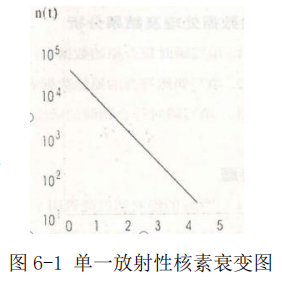
\includegraphics[scale=0.5]{t61}\end{center}

	由于实际上不能测到 t 时刻的计数率 n(t),测到的只能是某一时间间隔$\triangle t=t_2-t_1$的计数 N,再由 $N/\triangle t$ 求得平均计数率$\overline{n}$ ,$\overline{n}$ 和 n(t)的关系为
	\begin{equation}
	\overline{n}=\frac{1}{t_2-t_1} \int_{t_1}^{t_2}n(t)dt = \frac{n(0)}{\lambda (t_2-t_1)}(e^{-\lambda t_1}-e^{-\lambda t_2})
	\end{equation}
	可将n看作$t^{\prime}$时刻的计数率n($t^{\prime}$),即
	\begin{equation}
	n(0)e^{-\lambda t^{\prime}}=\overline{n}=\frac{n(0)e^{-\lambda t_1}[1-e^{-\lambda (t_2-t_1)}}{\lambda (t_2-t_1)}
	\end{equation}
	可得到$t^{\prime}$和$t_1$的关系为
	\begin{equation}
	t^{\prime}=t_1-\frac{1}{\lambda}ln\frac{1-e^{-\lambda (t_2-t_1)}}{\lambda (t_2-t_1)}
	\end{equation}
	在$\lambda \triangle t = \lambda(t_1-t_2) \gg 1$ 的条件下展开$)e^{-\lambda t}$ ,可得到
	\begin{equation}
	t^{\prime}=t_1-\frac{1}{\lambda}ln[1-\frac{1}{2}(\lambda \triangle t)+\frac{1}{6}(\lambda \triangle t)^2]
	\end{equation}
	进一步展开$ln(1-x)$ 可得
	\begin{equation}
	t^{\prime}=\frac{t_1+t_2}{2}-\frac{1}{24}\lambda \triangle t^2 \approx \overline{t}-0.0289 \times \triangle t \times (\frac{\triangle t}{T_{1/2}})
	\end{equation}
	若测量过程控制得好,使
	\begin{equation}
	0.0289 \times \triangle t \times (\frac{\triangle t}{T_{1/2}}) \gg \overline{t}
	\end{equation}
	就可以用n来表示$\overline{t}=\frac{t_1+t_2}{2}$时刻的计数率。在综合考虑上述简化原理和$\triangle t$测量时间中计数的统计误差后,选取适当的$\triangle t$,可以用$\overline{t}=\frac{t_1+t_2}{2}$代替$t^{\prime}$。

	\subsection{生产放射性核素的一般知识}
	将稳定核素 A 放在带电粒子或者中子流中辐照,产生核反应 $$ A+a \rightarrow B+b $$ 剩余核素 B 可能是放射性的。若剩余核素的衰变常数为$-\lambda$,则在恒定的入射粒子通量$\phi$下,放射性核素 B 活度 A(t)按
	\begin{equation}
	A(t)=\phi \sigma N_1 (1-e^{-\lambda t})
	\end{equation}
	规律生长,其中$\sigma$是该反应的反应截面(称为活化截面),Nt为样品中稳定核素A 的总数,$A(\infty)=\phi \sigma N_1$为饱和活度,表 1 给出了产生的活度和辐照时间 t 的关系。可以根据生产核素的半衰期和辐照条件权衡确定辐照吋间。
	\begin{center}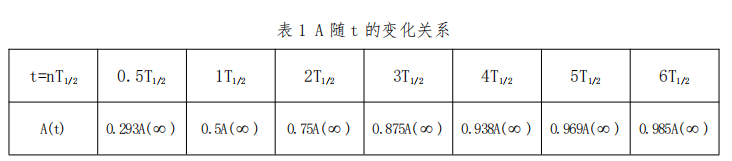
\includegraphics[scale=0.3]{b61}\end{center}

	天然铟的同位素丰富度及活化反应有关的数据列于表 2。当被激活样品中存在两种独立的放射性核素时,衰变曲线上的计数率是两种放射性核素的计数率之和
	\begin{equation}
	n(t)=n_1(t)+n_2(t)=n_1(0)e^{-\lambda_1 t}+n_2(0)e^{-\lambda_2 t}\label{hai}
	\end{equation}
	如图 6-1 表示。由总衰变曲线定出较长半衰期$(T_{1/2})_2$,然后从 n(t)中扣除$n_2(t)$,求出 $n_1(t)$,再得到$(T_{1/2})_1$。铟活化后生成五种放射性核素和同质异能素,由于同质异能素$^{116m}In$的半衰期和其他四种放射性核素半衰期相差 1-2 个数量级以上,适当选择活化辐照时问和“冷却时间”(即从停止辐照到开始测量活性的时间),可以使其它四种放射性对$^{116m}In$ 半衰期测量的影响很小,故而可以用单一放射性半衰期的规律处理数据。
	\begin{center}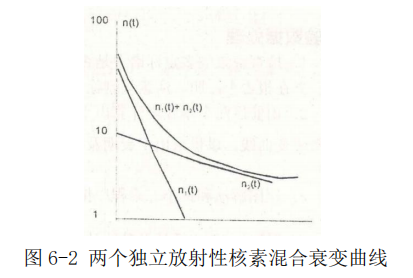
\includegraphics[scale=0.5]{t62}\end{center}
	\begin{center}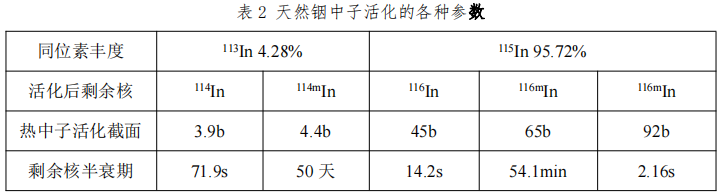
\includegraphics[scale=0.3]{b62}\end{center}

	\section{实验结果}
	前后两个本底段计算出平均本底计数分别为19.83 ,20.33 。总平均20.08 ,取20 。

	\subsection{图解法}
	由于实验中中子活化后立即开始了测量,我们去除前九分钟的数据。考虑到外界干扰,已删除不合理的过高计数。对所测粒子数取对数作图如下所示
	\begin{center}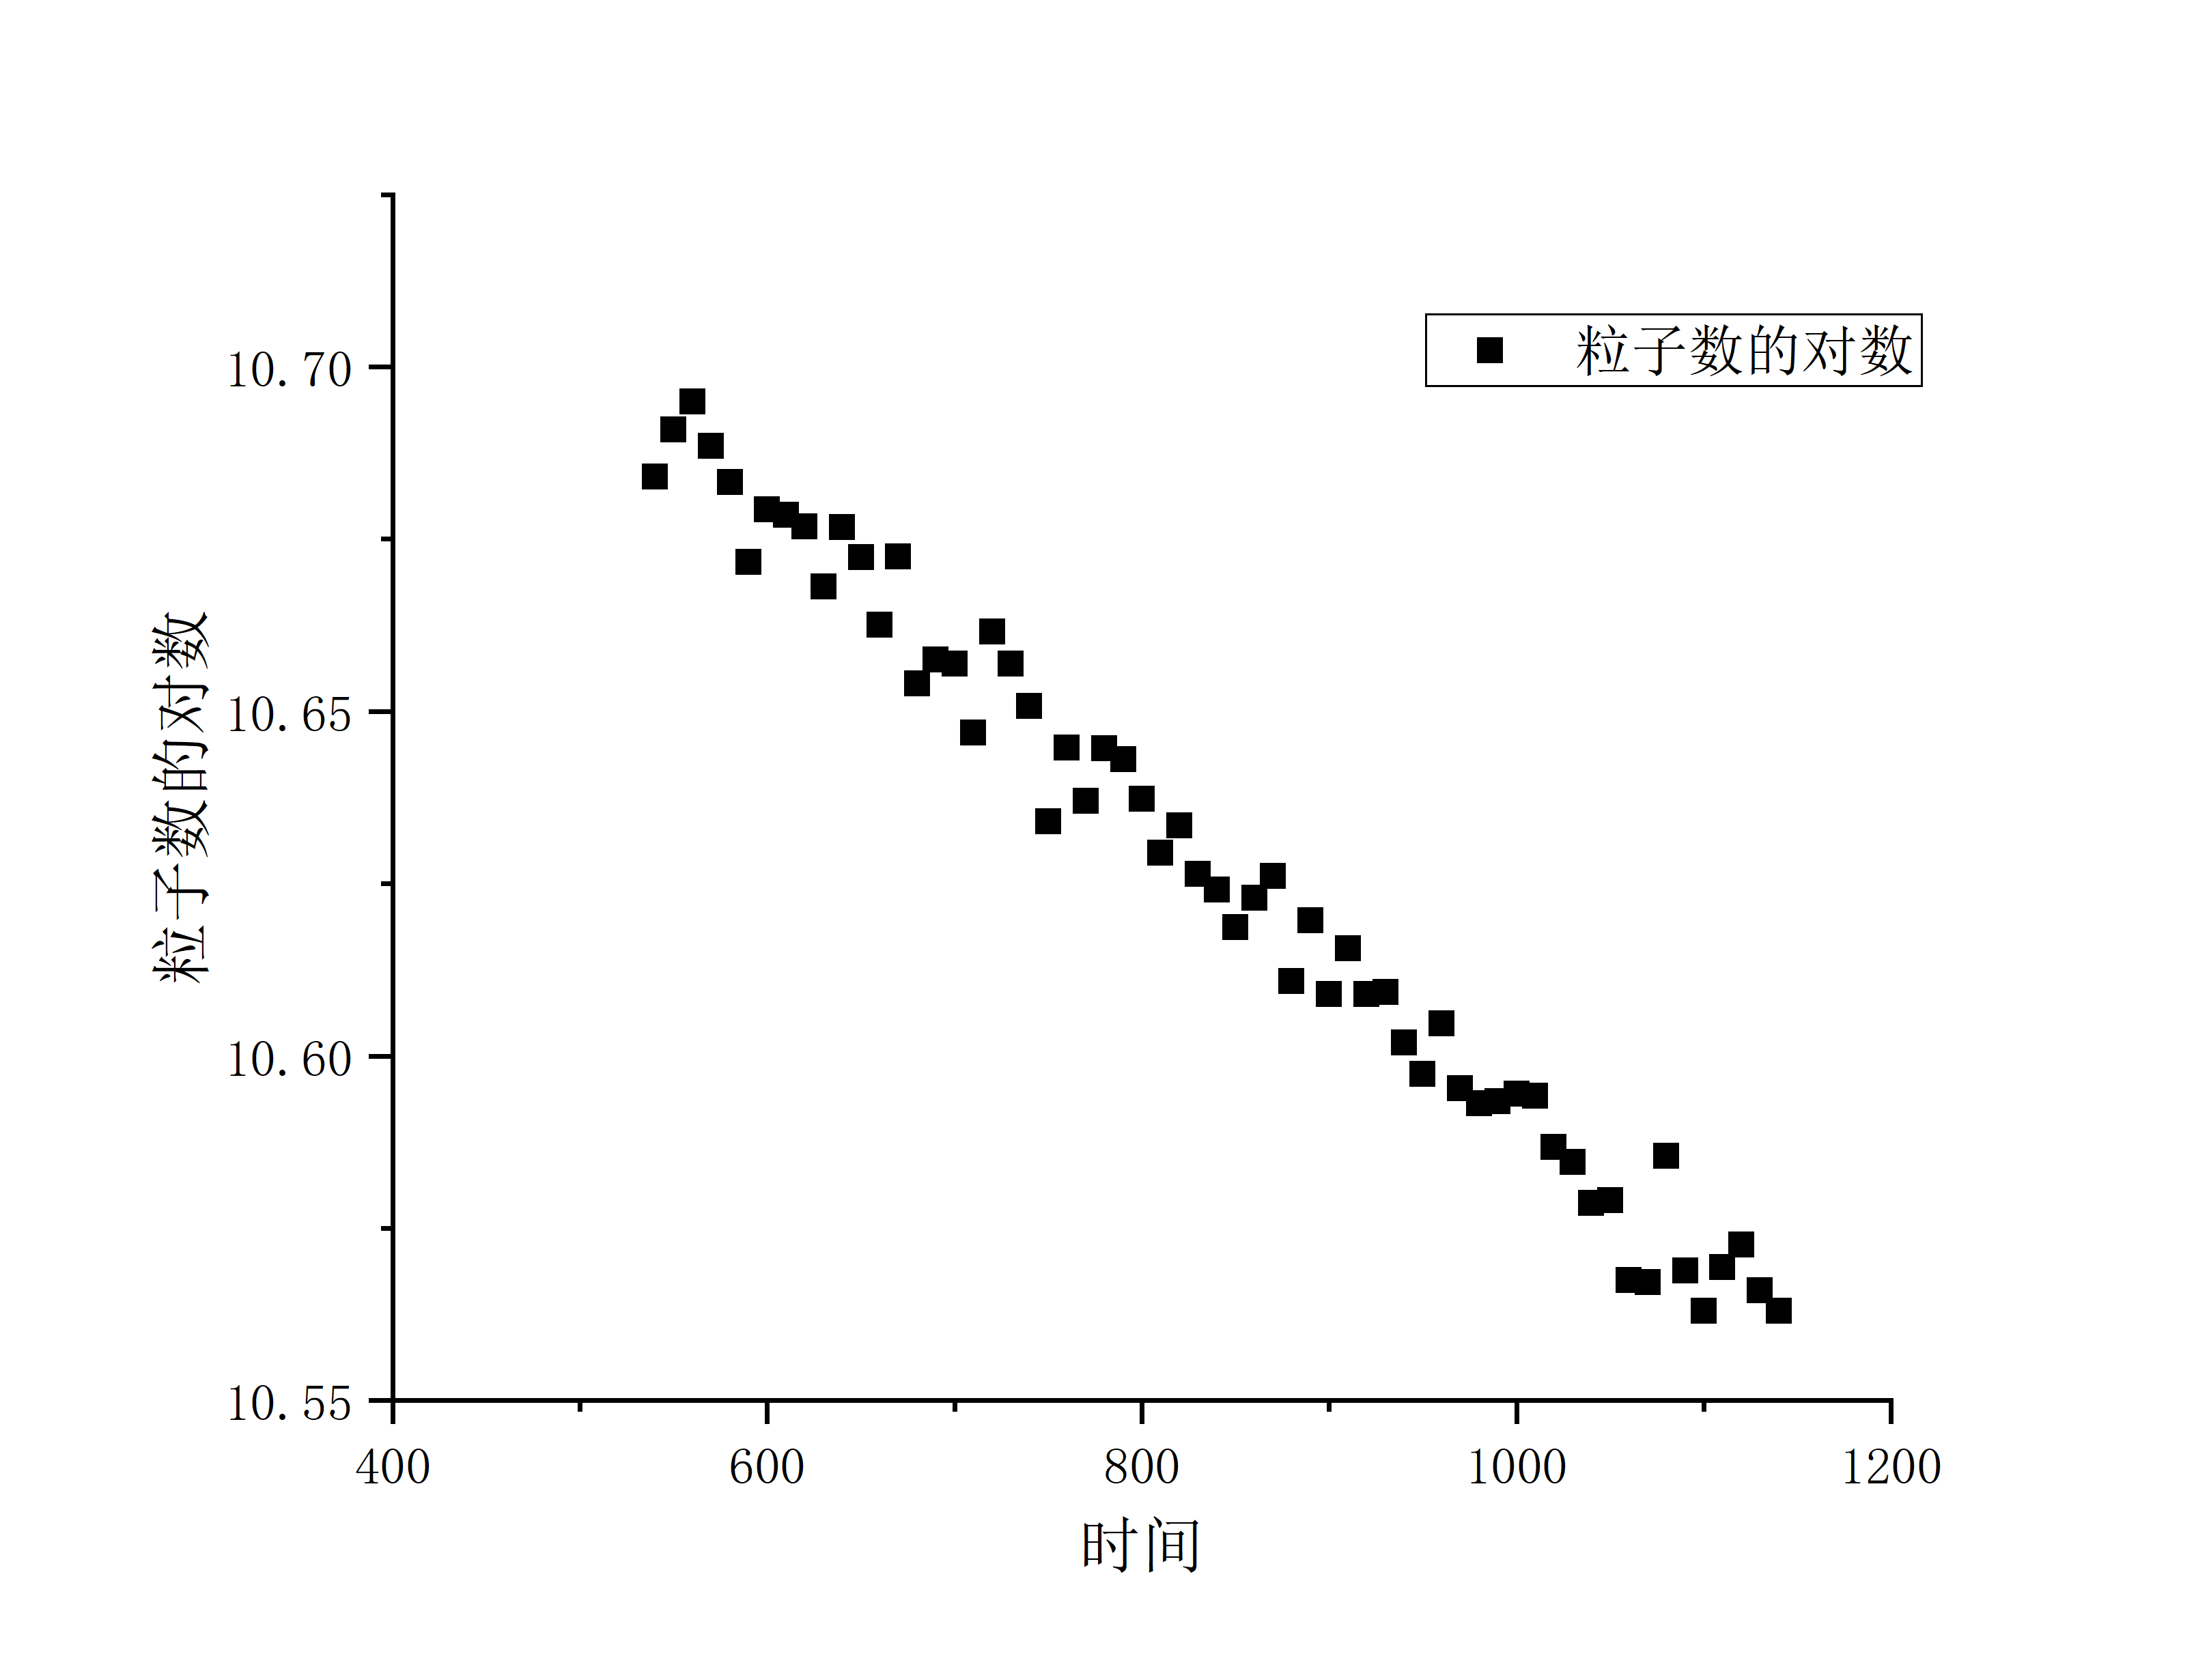
\includegraphics[scale=0.3]{t2}\end{center}
	
	通过目测,可知其斜率大约是$2.2 \times 10^{-4}$,利用式\eqref{chu}可知其半衰期为52.5分钟。

	\subsection{最小二乘法}
	运用公式
	\begin{equation}
	y=y_0+Ae^{-x/t_0}
	\end{equation}
	其中,半衰期$T_{1/2}=t_0ln2$。用Origin拟合结果如下图所示
	\begin{center}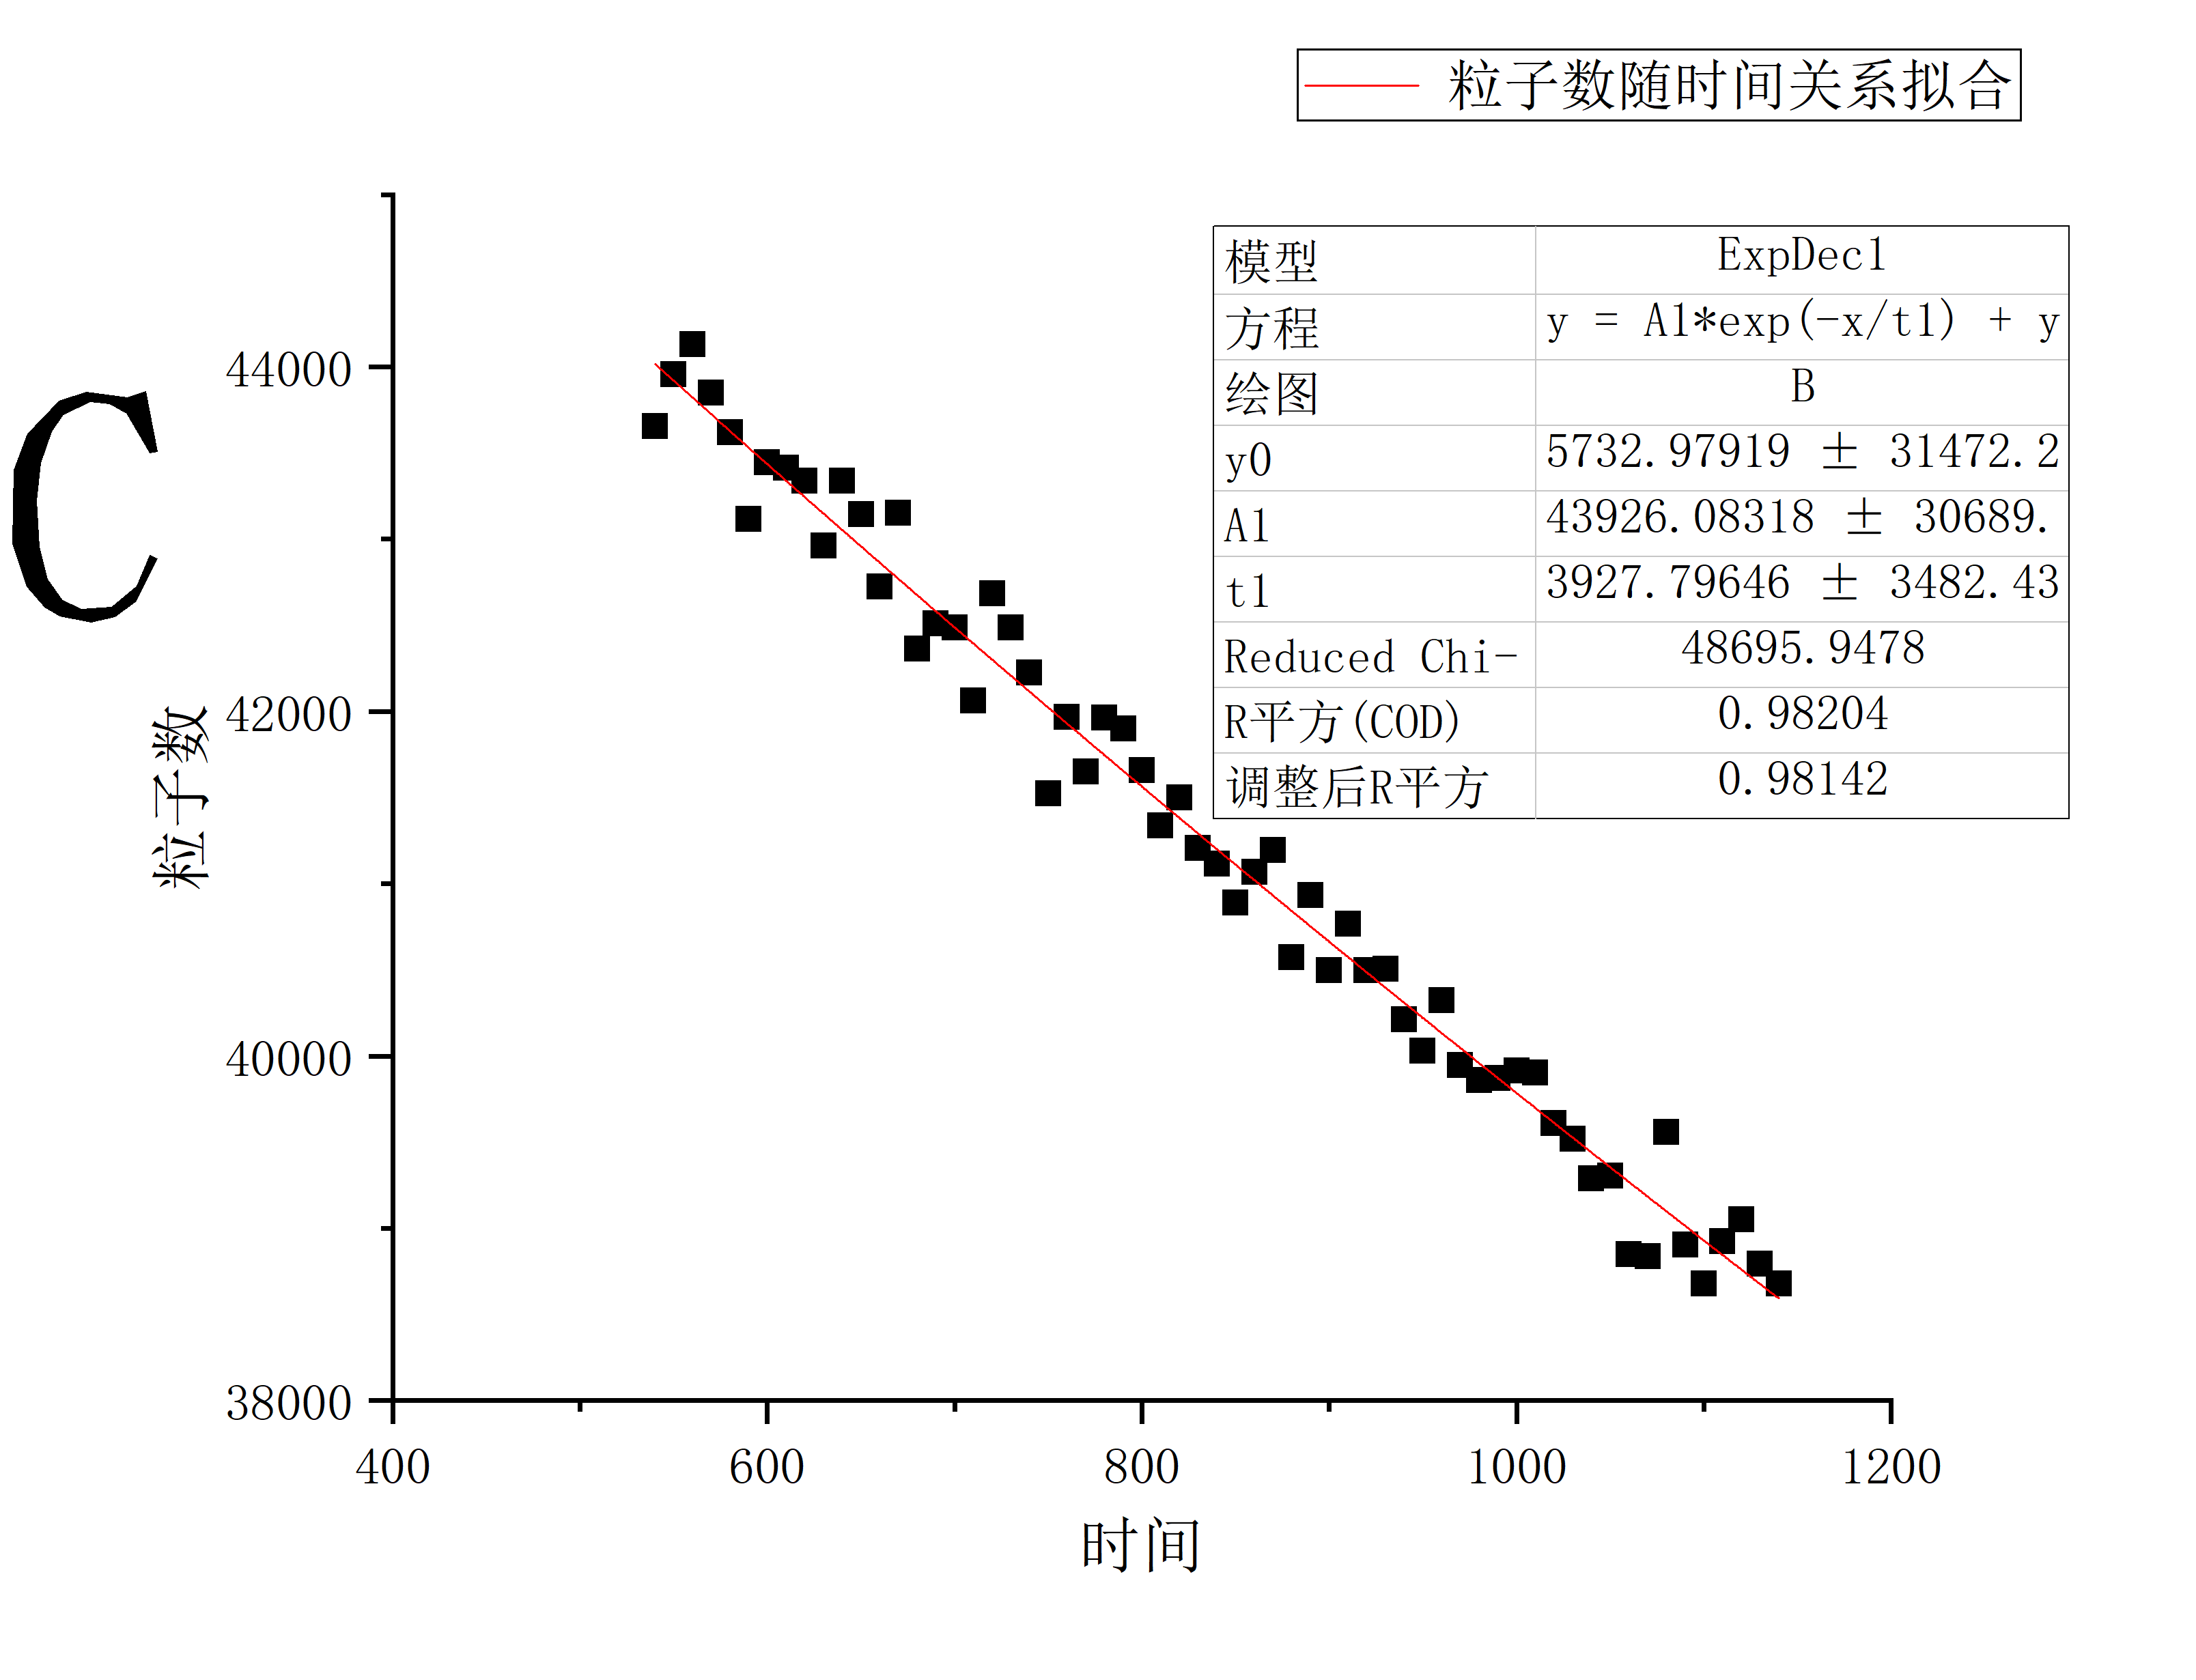
\includegraphics[scale=0.3]{t3}\end{center}

	可以算出半衰期及其误差$T_{1/2} \pm \triangle T_{1/2}=45\pm40$分钟。

	可见其误差过大,考虑到实验设备涨落太大而所选实验数据太少。我们结合$In$的衰变原理,只去除前一分钟的数据,把$^{114}In$的放射也考虑进来,使用下式进行拟合
	\begin{equation}
	y=y_0+A_1e^{-x/t_1}+A_2e^{-x/t_2}
	\end{equation}
	\begin{center}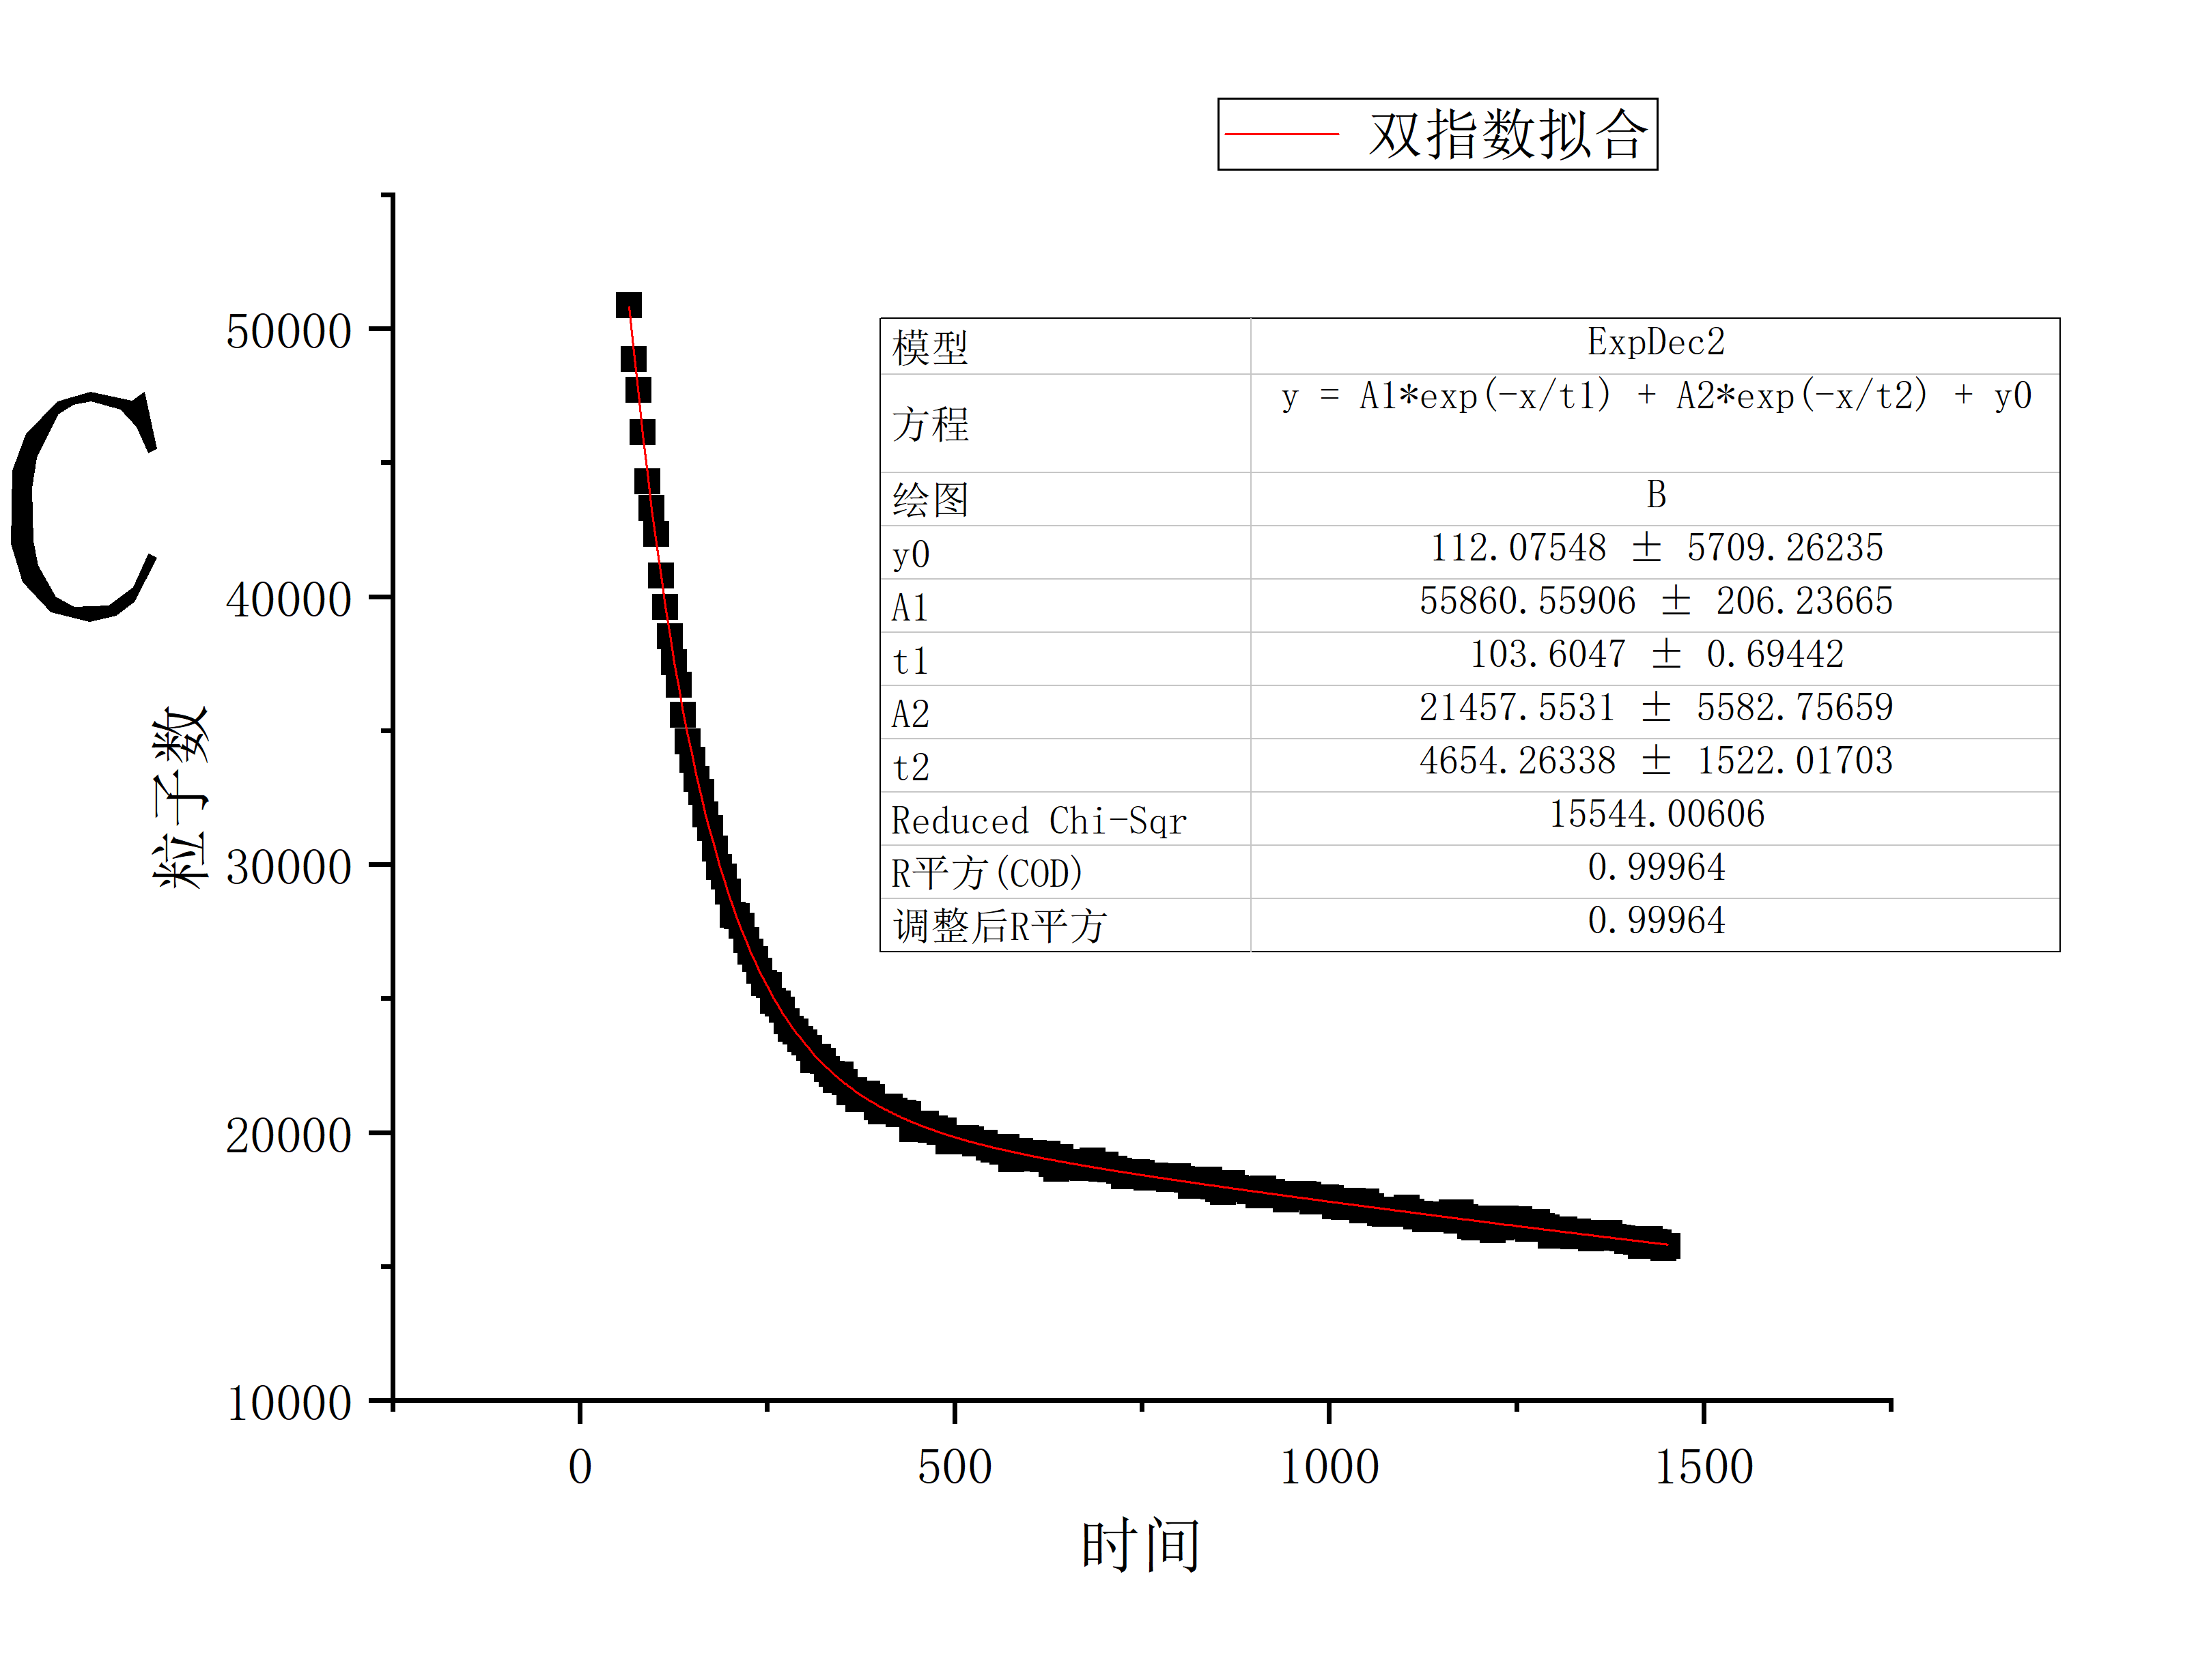
\includegraphics[scale=0.3]{t32}\end{center}
	如上图所示,可知$In$半衰期及其误差$T_{1/2} \pm \triangle T_{1/2}=54 \pm 18$分钟。本底的误差相对这个值很小,我们忽略不计。

	\subsection{间断多定标谱}
	活性测量间隔为 3 道,二次活性测量时间间隔为 5 道,起始测量时间为 80 道。
	两次测量图解法如图
	\begin{center}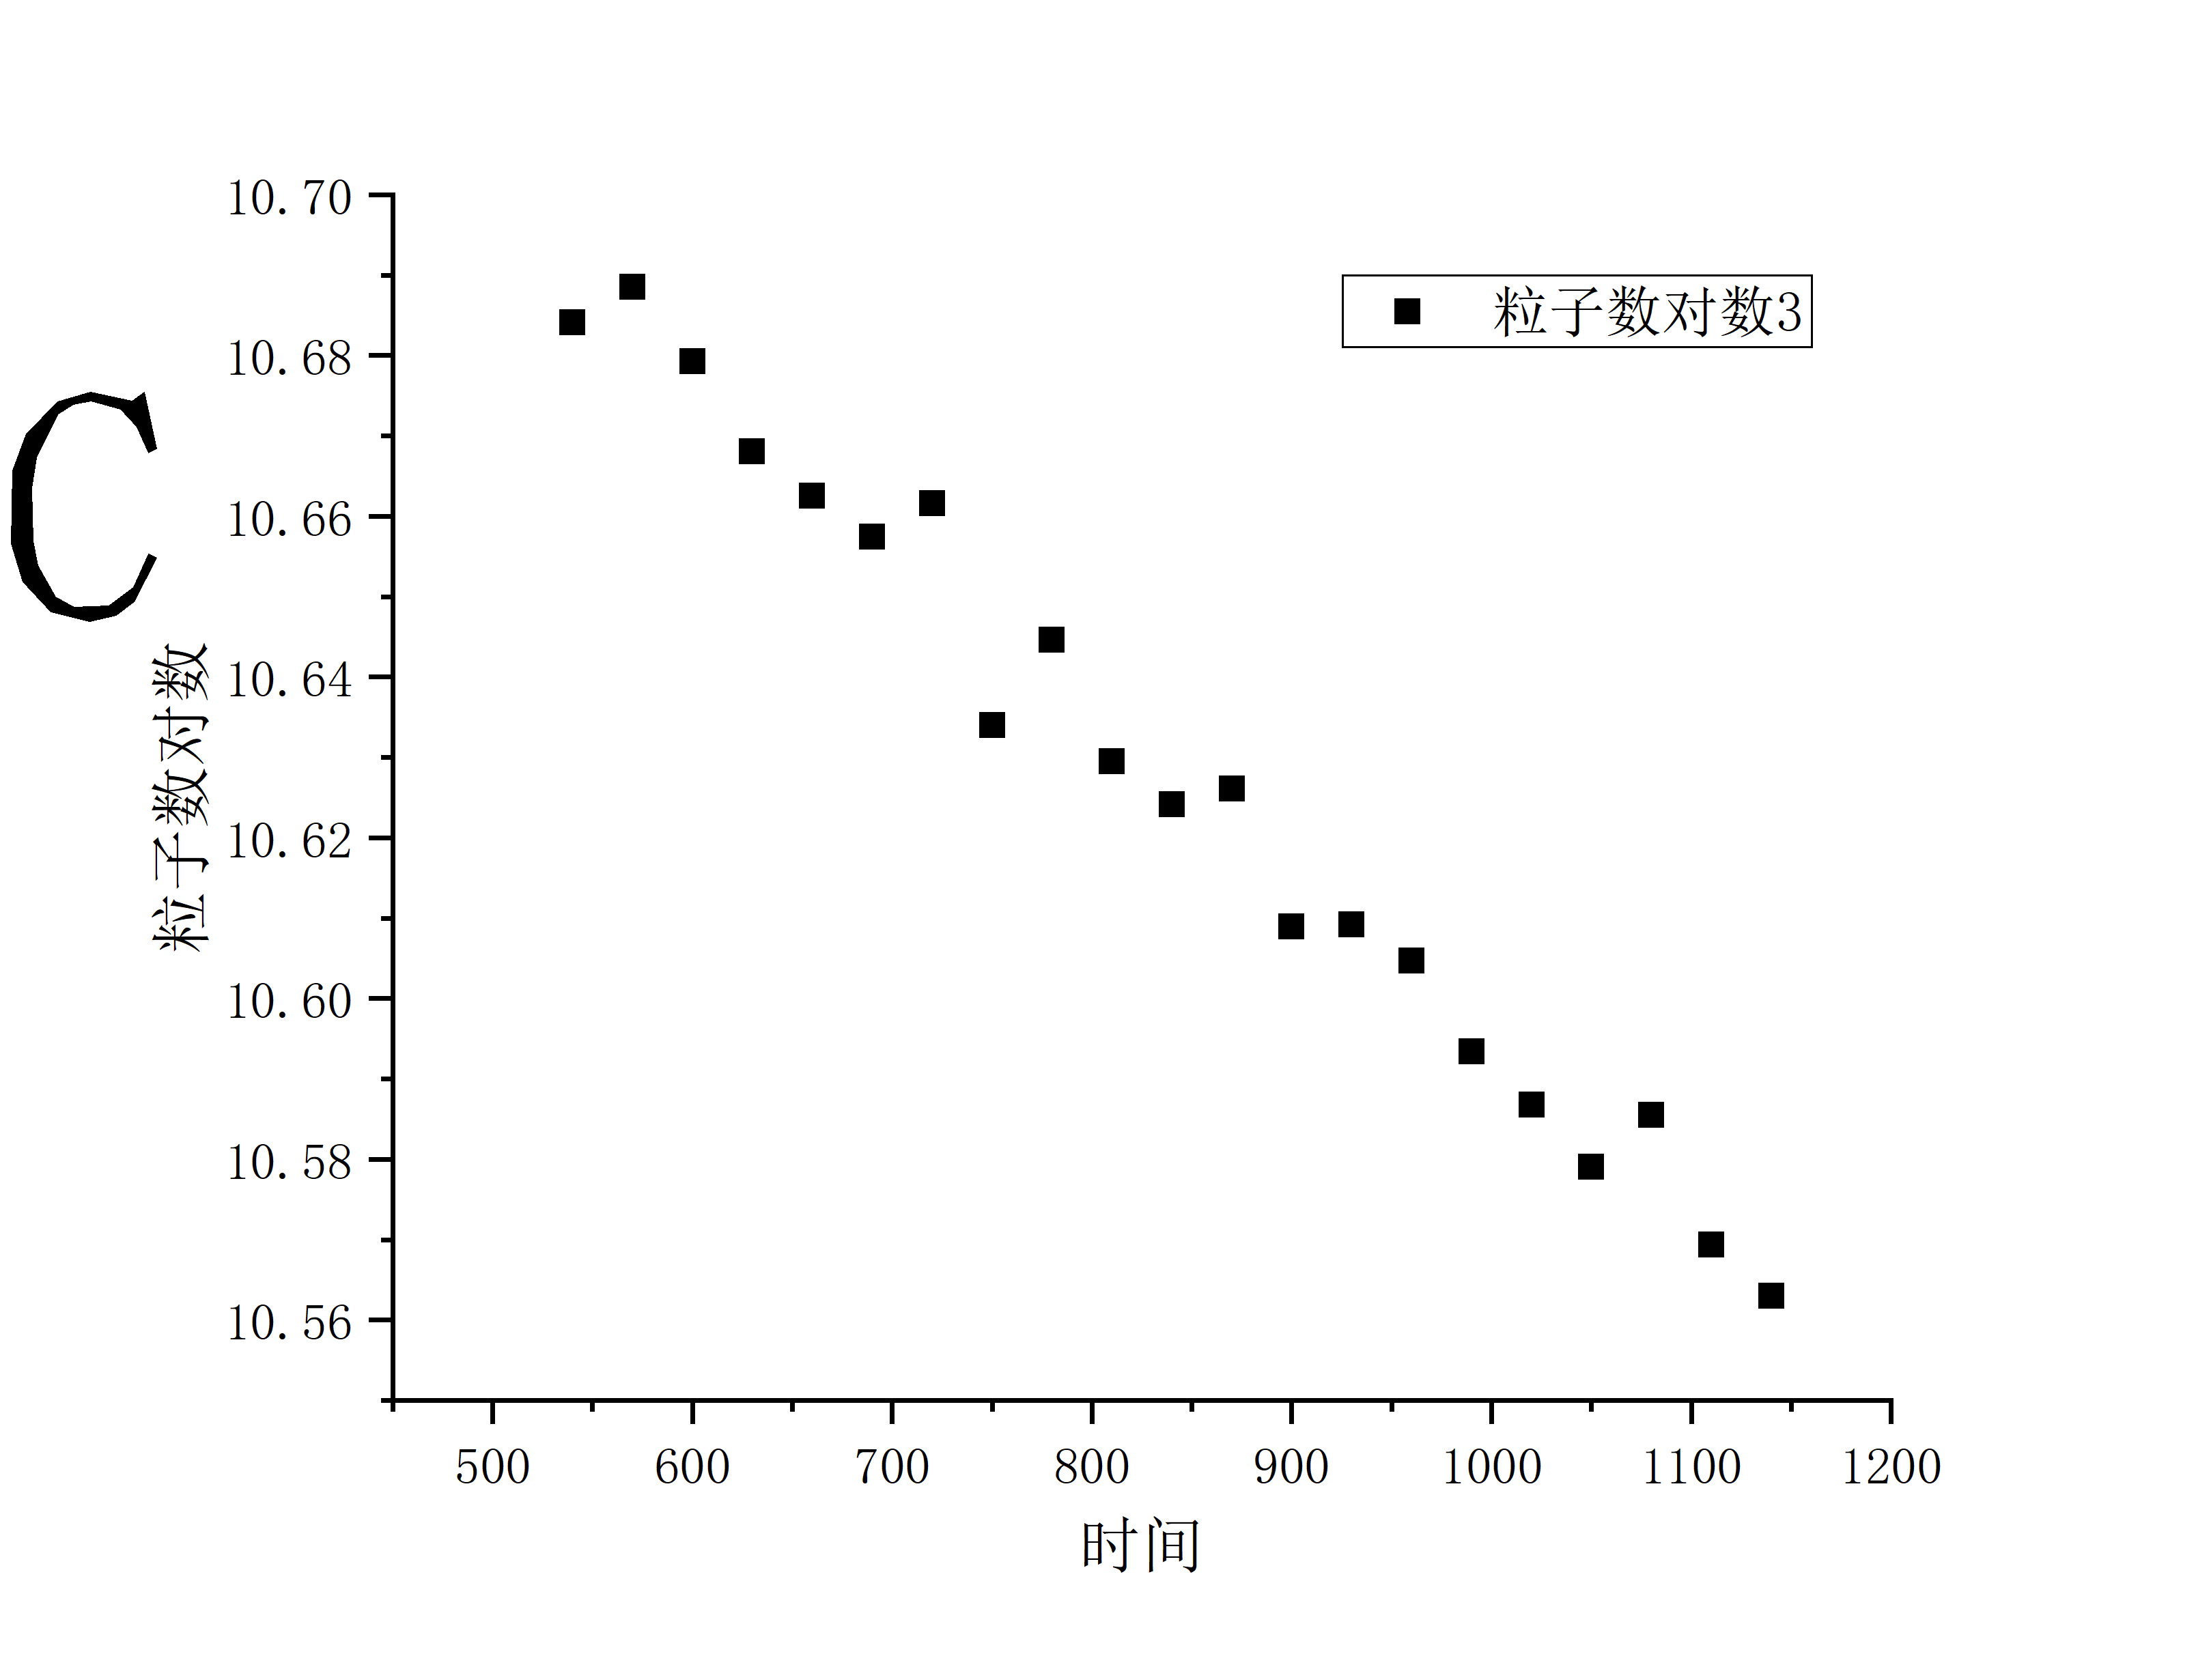
\includegraphics[scale=0.3]{t41}\end{center}
	\begin{center}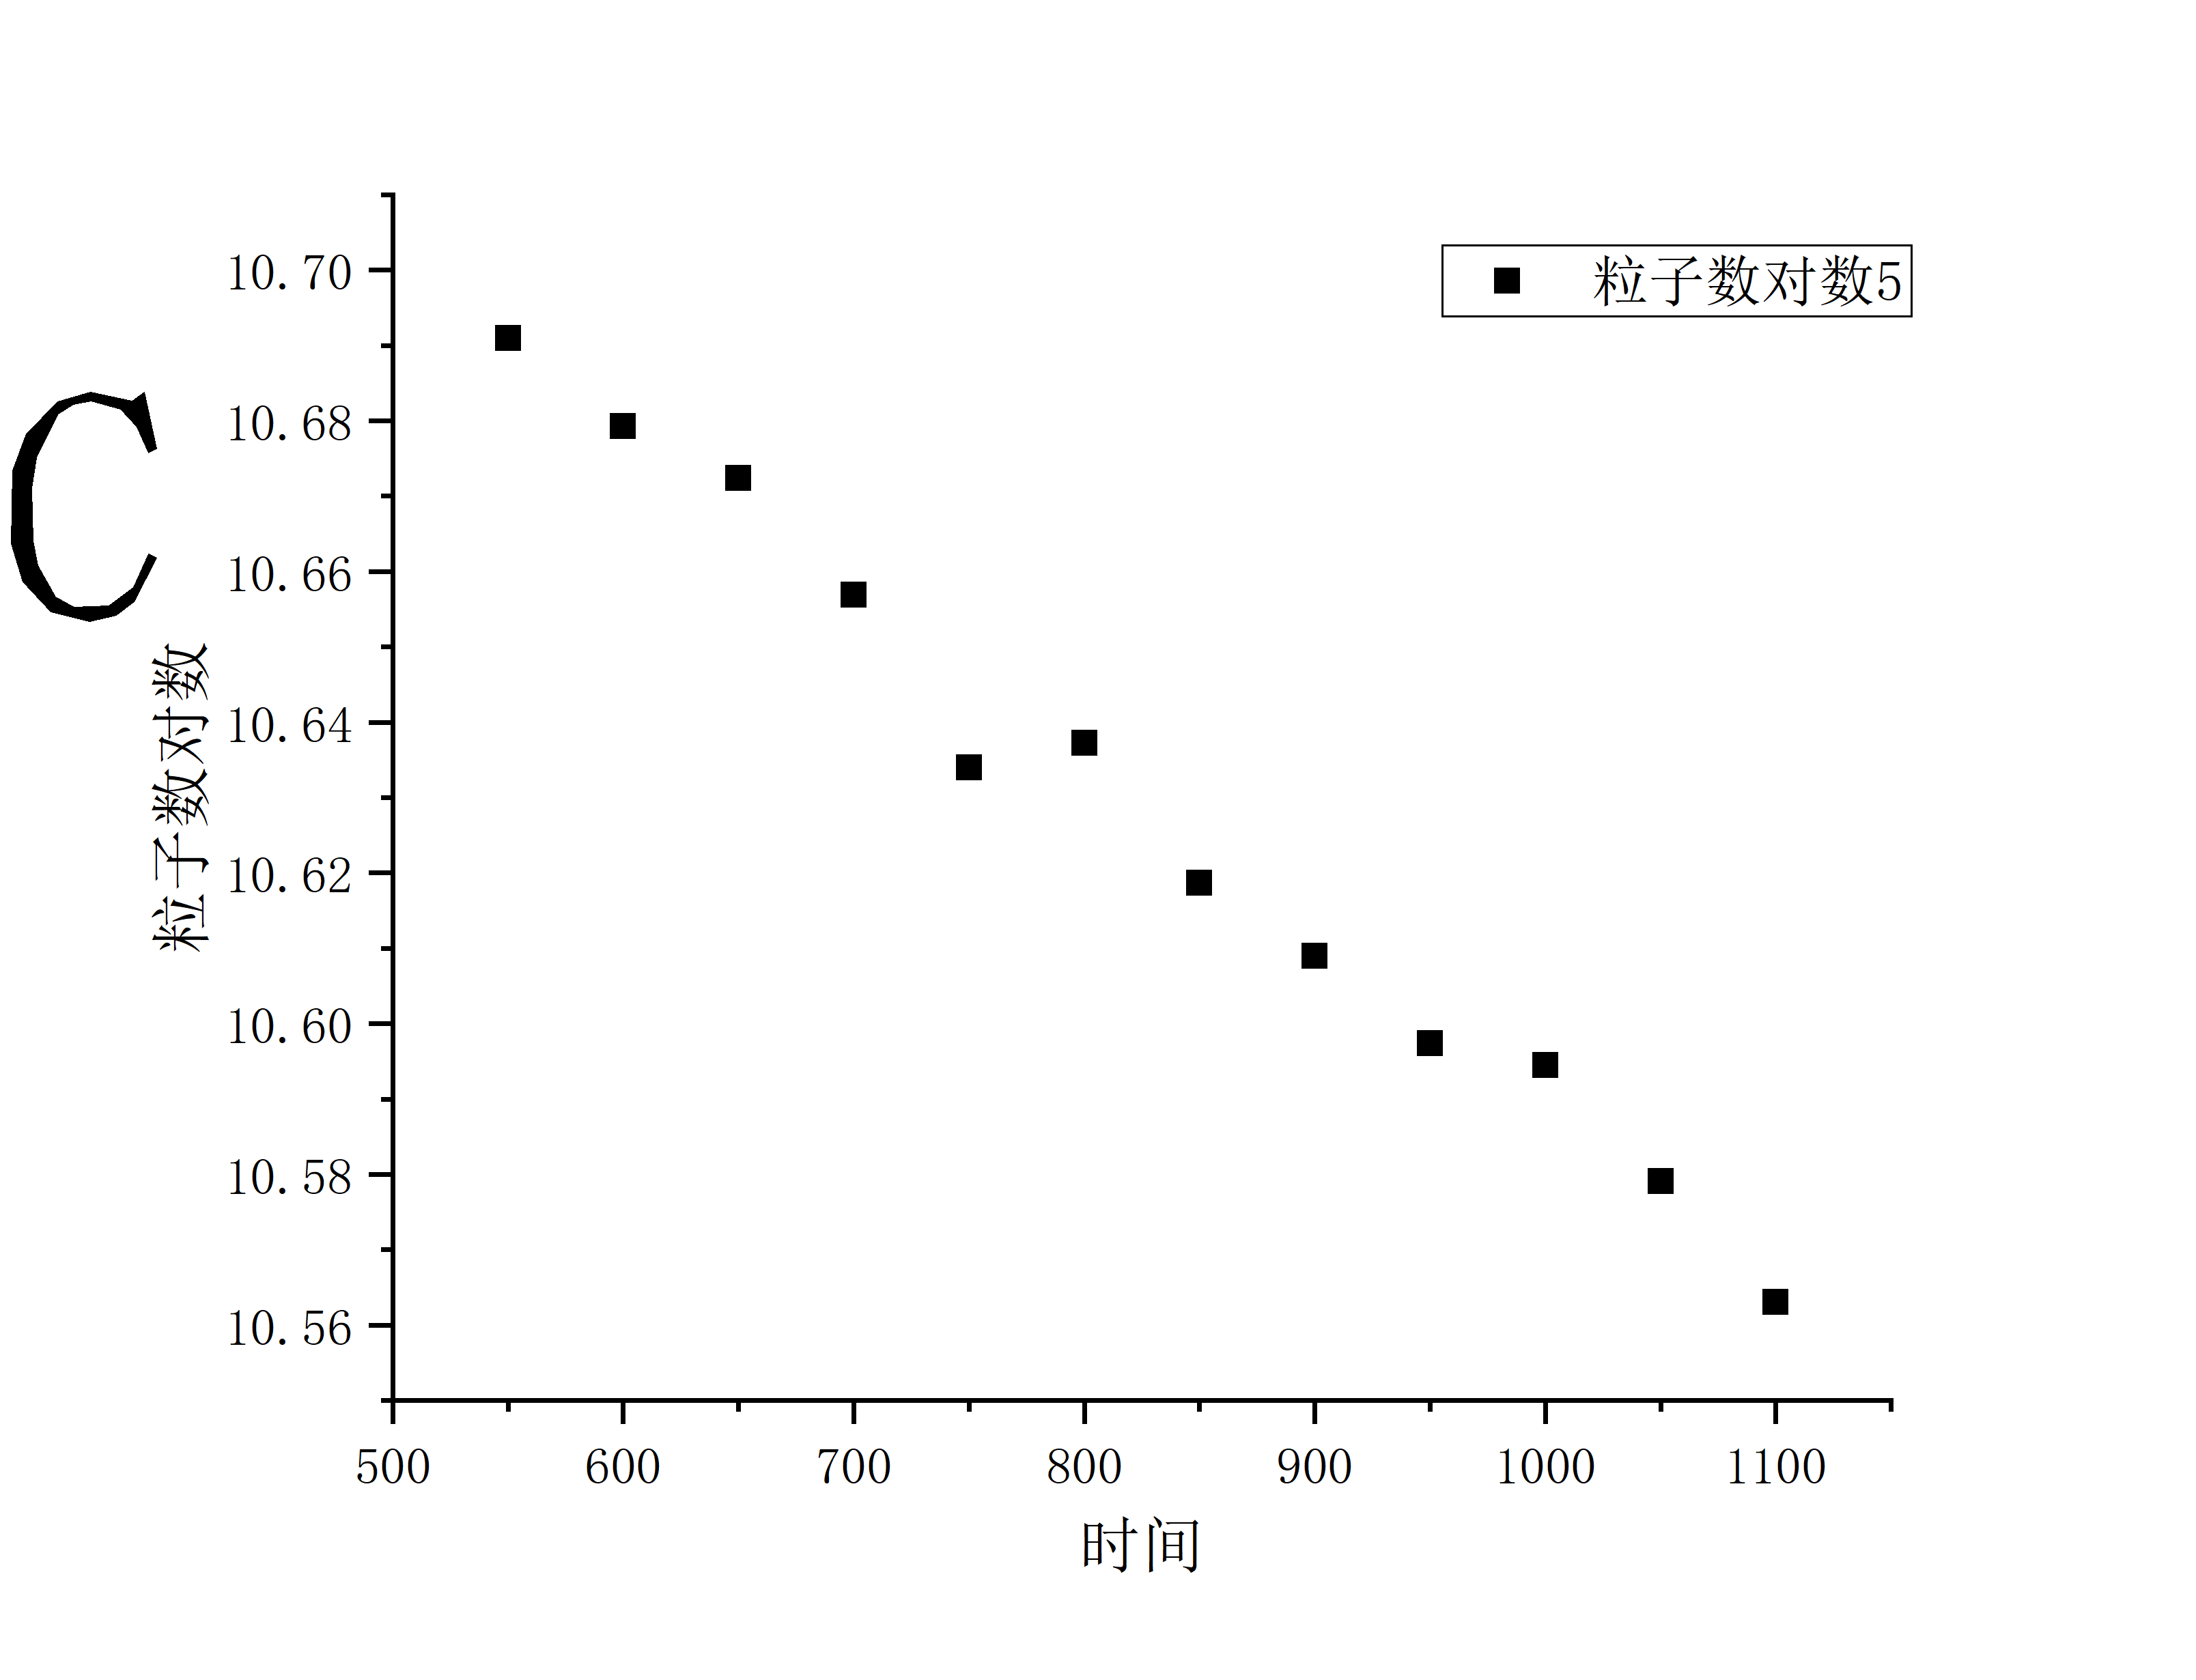
\includegraphics[scale=0.3]{t43}\end{center}
	两次次斜率分别为$2.17 \times 10^{-4}$,$2 \times 10^{-4}$。利用式\eqref{chu}分别求其半衰期为53.3分钟、57.8分钟。

	活性测量间隔为 3 道,二次活性测量时间间隔为 5 道,起始测量时间为 10 道。
	双指数拟合如下图所示
	\begin{center}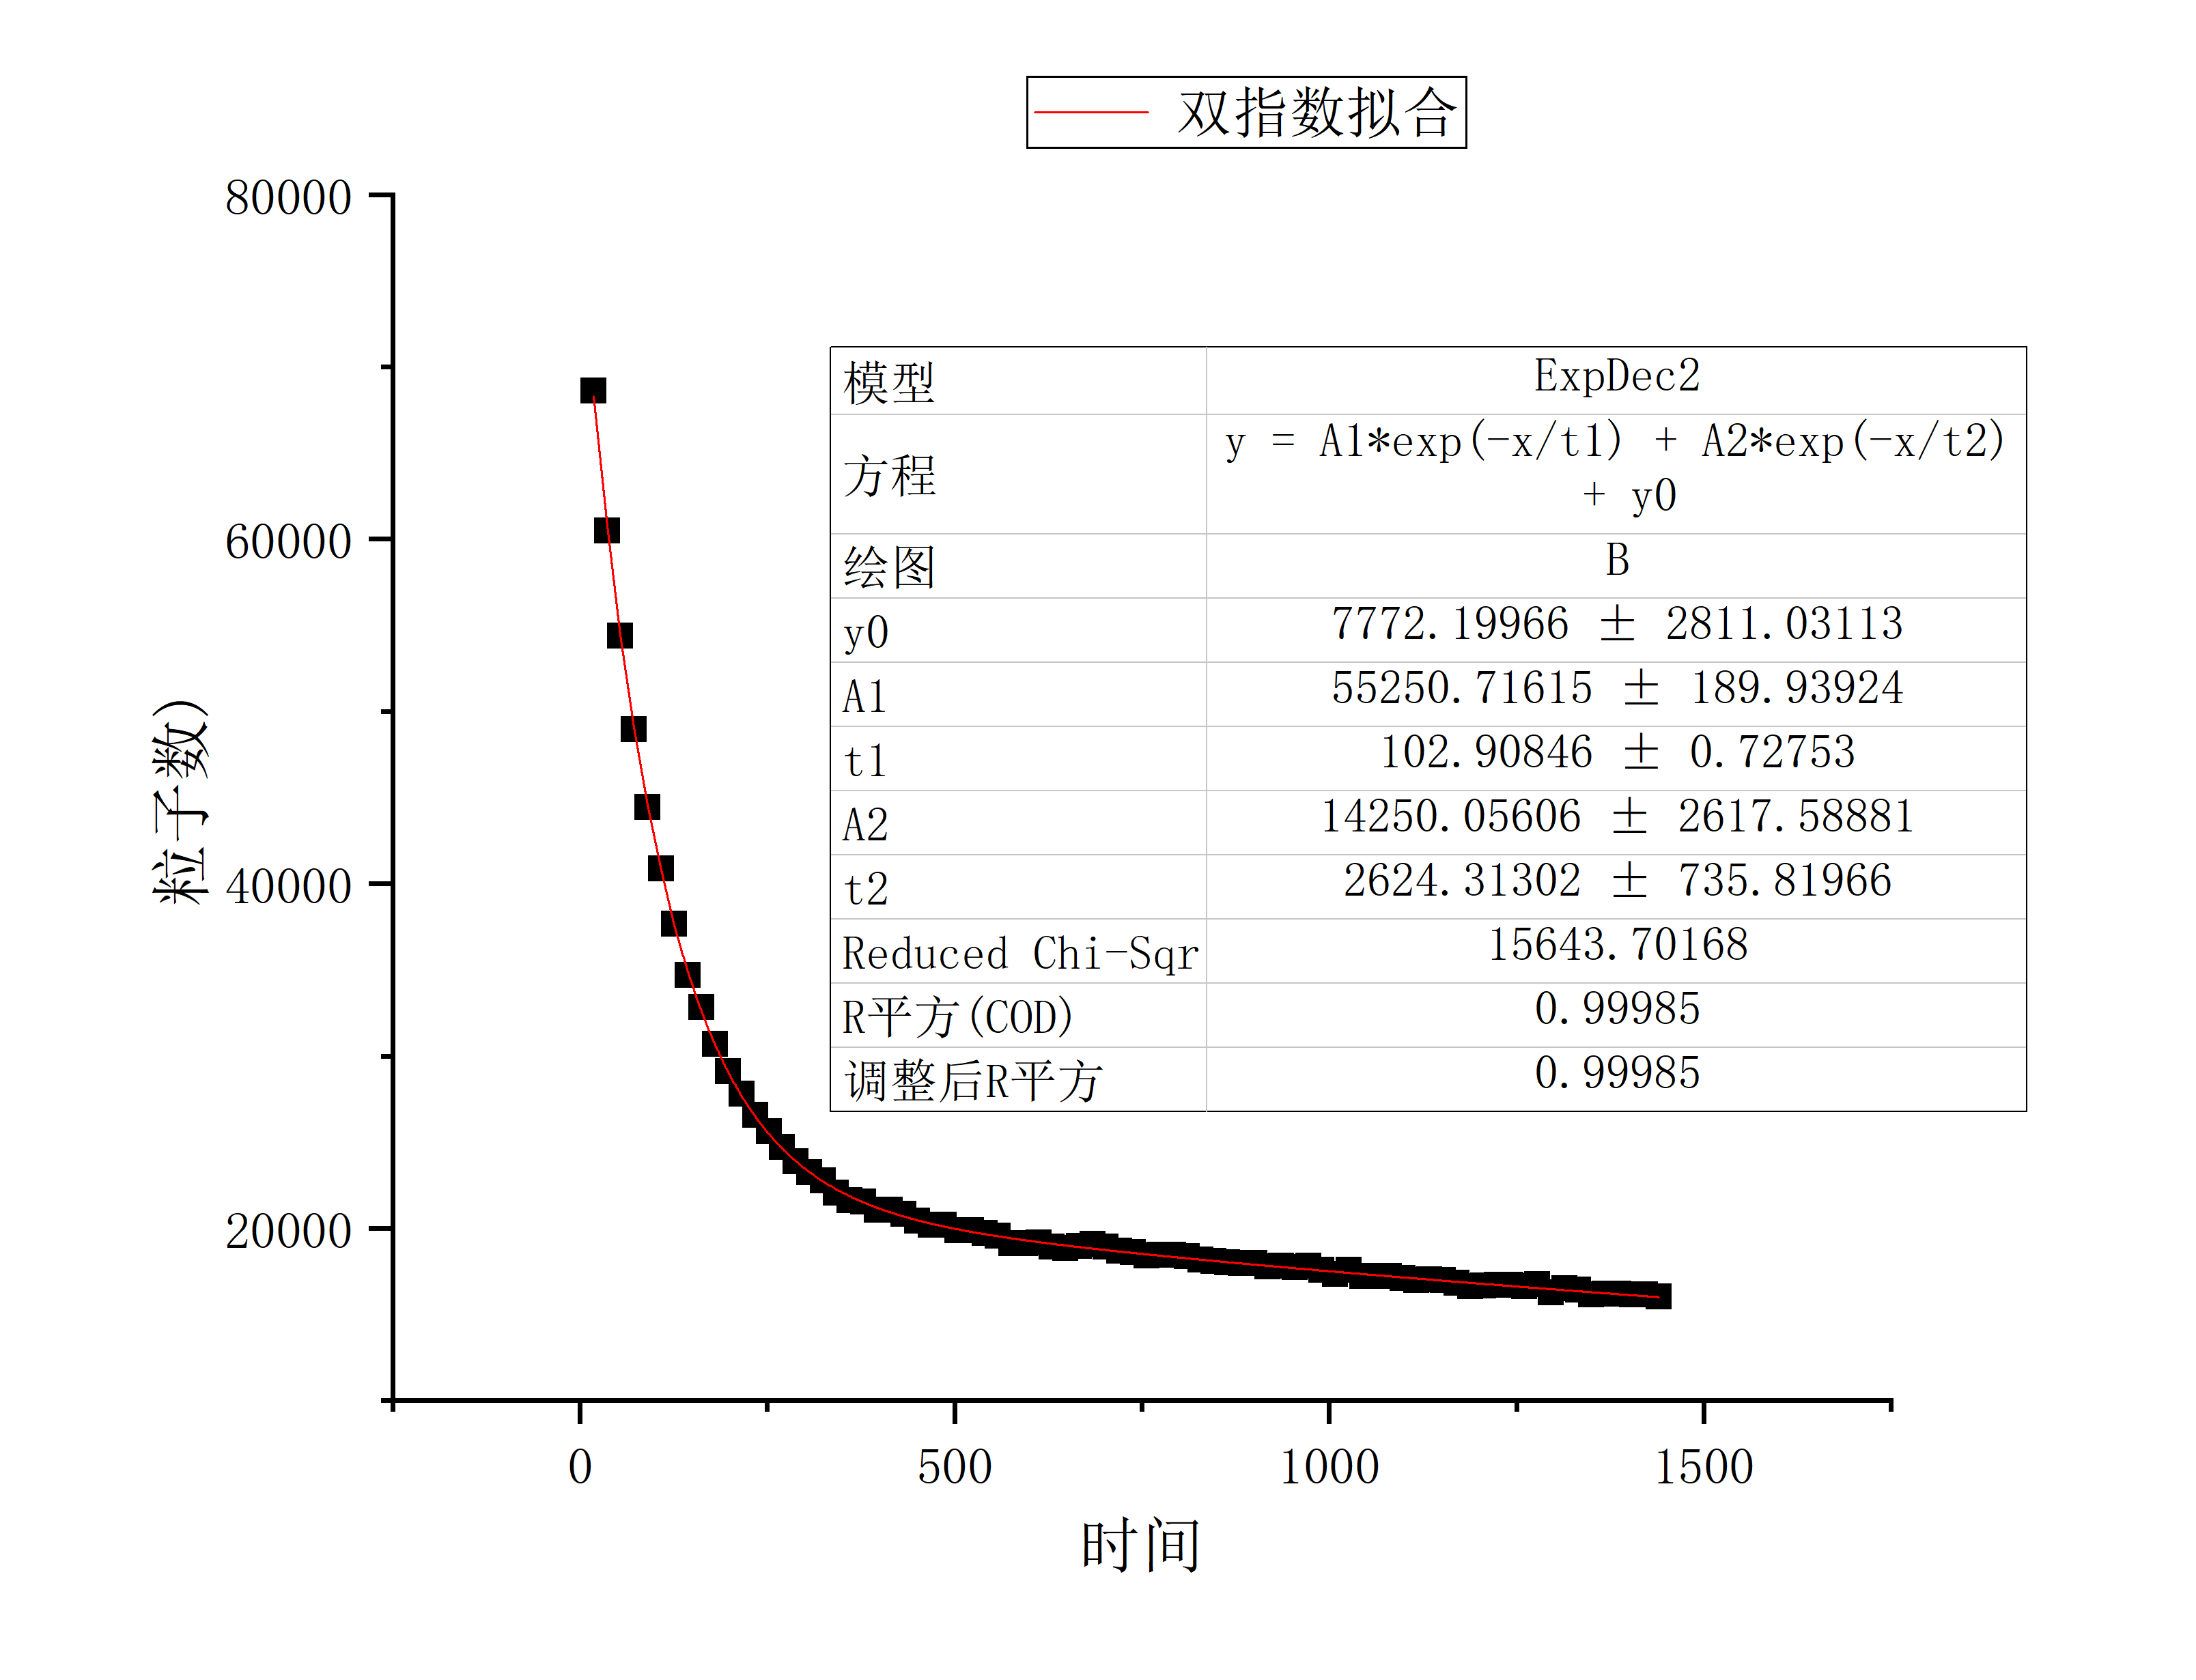
\includegraphics[scale=0.3]{t42}\end{center}
	\begin{center}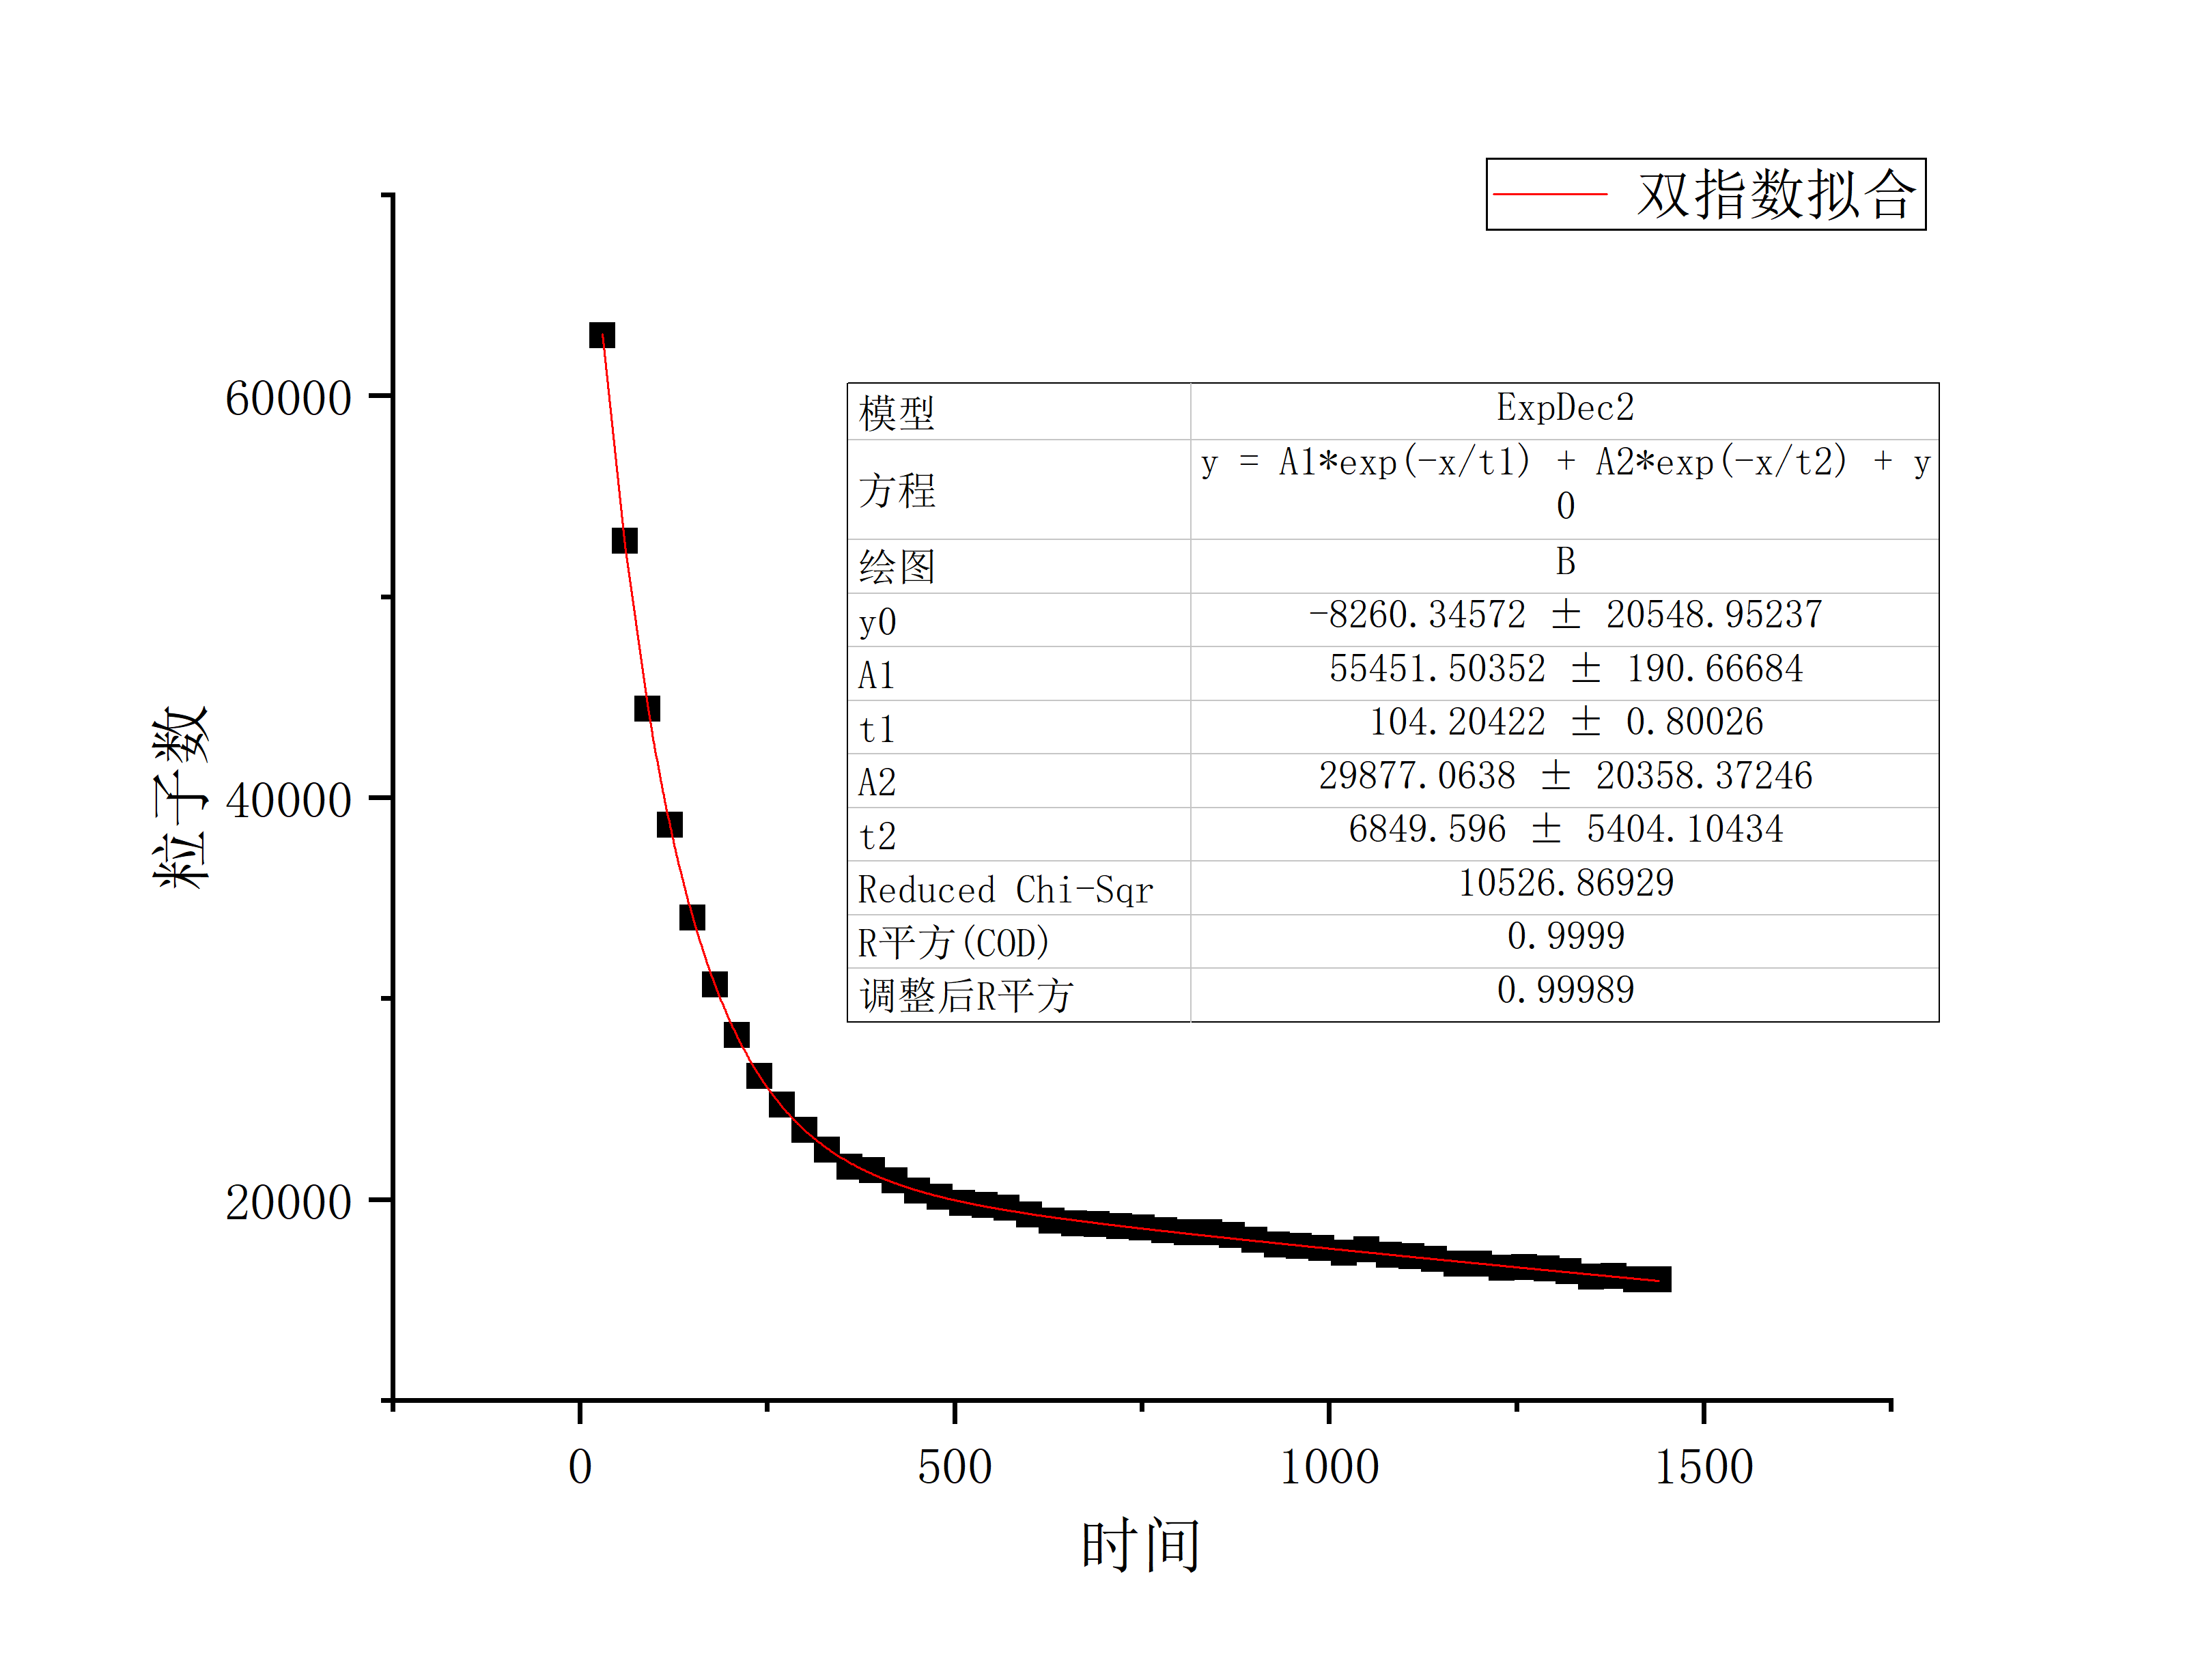
\includegraphics[scale=0.3]{t44}\end{center}
	可以算出半衰期及其误差$T_{1/2} \pm \triangle T_{1/2}=43 \pm 12$分钟和$79 \pm 62$分钟。属实不能随便删点,虽然54仍然在区间之内,但误差太大。

	第一道和最后一道不取是因为开始测量可能产生干扰场,对数据影响较大。

	\section{讨论}
	\subsection{单一半衰期处理的可靠性}
	取活化时间为 3 个$^{116m}In$ 半衰期,即162.3min。由表1及式\eqref{hai}分别计算$In$活度,注意到$^{114}In$近乎完全激活,设其活度为$3.9\times 0.0428 = 0.16692$。依次得$^{114m}In$活度0.010 ,$^{116}In$活度43.074 ,$^{116m}In$活度54.4408 和88.0624 。

	由表2,我们直接以相对活度求差,$t \in (10min,118.2min)$。
	\begin{equation}
	A =2^{-\frac{t_2}{T_{1/2}}}-2^{-\frac{t_2}{T_{1/2}}}
	\end{equation}
	
	依次求得:$^{114}In$所占活性为$5.1 \times 10^{-4}$,$^{114m}In$所占活性为$1.0 \times 10^{-5}$,$^{116}In$所占活性为$8.2 \times 10^{-12}$,$^{116m}In$所占活性为$35.88979$和$2.1 \times 10^{-82}$。

	那么实验所测$^{116m}In$活性占比为99.9985\%。

	\subsection{具体措施}
	增加了铅片,屏蔽了一些外界干扰。测量多道,减少统计误差。$\lambda \triangle t = \lambda(t_1-t_2) \gg 1$ 的条件下,可以用$\overline{t}=\frac{t_1+t_2}{2}$代替$t^{\prime}$。

	测量了两次本底取平均值,减少误差。在衰变曲线中扣除了本底。本身误差比较大,所以本底误差没那么重要。























\end{multicols}
\end{document}